\PassOptionsToPackage{dvipsnames}{xcolor}

\documentclass[12pt]{beamer}
\usetheme{default}
\usecolortheme{crane}

\usepackage[T1]{fontenc}
\usepackage[slovak]{babel}

\usepackage{amsmath}
\usepackage{amsmath, amssymb}
\usepackage{hyperref, url}
\usepackage{graphicx}
\usepackage{array}
\usepackage{alltt}
\usepackage{tikz}

%\setbeamersize{text margin left=1pt,text margin right=1pt}
\setbeamertemplate{footline}[frame number]
\beamertemplatenavigationsymbolsempty

% https://www.overleaf.com/learn/latex/Using_colours_in_LaTeX
\def\blue#1{\textcolor{Cerulean}{#1}}
\def\green#1{\textcolor{LimeGreen}{#1}}

% database-related stuff
\DeclareMathOperator{\join}{\bowtie}
\DeclareMathOperator{\antijoin}{\rhd}

\DeclareMathOperator{\lubi}{lubi}
\DeclareMathOperator{\capuje}{capuje}
\DeclareMathOperator{\navstivil}{navstivil}
\DeclareMathOperator{\vypil}{vypil}
\DeclareMathOperator{\answer}{answer}

\title{Transakcie}
\author{Ján Mazák}
\institute{FMFI UK Bratislava}
\date{}


\begin{document}

\frame{\titlepage}


\begin{frame}[fragile]{Transakcie}
\alert{Transakcie}, ktoré sa vykonajú celé, alebo vôbec nič z nich:
\begin{itemize}
\item riešia konzistenciu dát z hľadiska používateľov databázy;
\item riešia problém so zlyhaniami\\ (hardvér, výpadky siete či elektriny);
\item môže ich paralelne prebiehať mnoho,\\ navzájom o sebe nevedia.
\end{itemize}

\bigskip
Operácie v rámci transakcie:
\begin{itemize}
\item start (BEGIN TRANSACTION)
\item read (SELECT)
\item write (INSERT, UPDATE, DELETE)
\item \blue{COMMIT} (úspešné ukončenie) /\\\green{ROLLBACK} (abort, zrušenie)
\end{itemize}
\end{frame}


\begin{frame}[fragile]{Transakcie}
Príklad transakcie (PostgreSQL):
\begin{alltt}
    BEGIN;
    UPDATE accounts SET balance = balance - 100.00
        WHERE name = 'Alice';
    UPDATE accounts SET balance = balance + 100.00
        WHERE name = 'Bob';
    COMMIT;
\end{alltt}
DBMS je jedno, že sa nejaké peniaze stratia, ale musí autorovi SQL príkazov umožniť, aby sa tomu vedel vyhnúť.
\end{frame}


\begin{frame}[fragile]{Transakcie}
Príklad transakcie (Python):
\begin{alltt}
    command = 'INSERT INTO student VALUES (\%s, \%s)'
    cursor = conn.cursor()
    cursor.execute(command, ('a', 'b'))
    cursor.execute(command, ('c', 'd'))
    conn.commit()
\end{alltt}
(psycopg; sqlite3 používa namiesto \%s znak ?)
Príkaz pre začiatok transakcie sa odošle automaticky.
Databázové drivery zväčša umožňujú nastaviť tzv. \emph{autocommit} mód,
keď je každý vykonávaný príkaz transakciou sám osebe.
(Pozor: autocommit je neraz nastavený ako default.)
\end{frame}


\begin{frame}[fragile]{Transakcie}
Za prelínanie jednotlivých transakcií zodpovedá \blue{scheduler},
ktorý vytvára \alert{rozvrh} obsahujúci jednotlivé operácie (tiež \alert{história}).
Scheduler nevidí do budúcnosti a pre každú požiadavku jednotlivých transakcií
musí ihneď rozhodnúť, čo~s~ňou:
\begin{itemize}
\item vykonať hneď
\item počkať a skúsiť požiadavku zaradiť neskôr
\item abortnúť transakciu (napr. ak sa požiadavka nebude dať vykonať ani v budúcnosti, alebo ako prevenciu deadlocku)
\end{itemize}
\end{frame}


\begin{frame}[fragile]{Transakcie}
Dôvody abortu transakcie:
\begin{itemize}
\item explicitné želanie klienta
\item výpadok na strane klienta
\item výpadok na strane servera
\item strata spojenia medzi klientom a serverom
\item scheduler usúdi, že nie je možné v transakcii pokračovať\\
    (napr. by došlo k neriešiteľnému konfliktu s inou tx)
\end{itemize}
Klient musí počítať s tým, že dôjde k abortu jeho transakcie, aj keď všetko vykonal správne.
\end{frame}


\begin{frame}[fragile]{Požiadavky na transakčný systém --- ACID}
\begin{itemize}
\item \green{A}tomicity --- tx sa vykoná celá, alebo vôbec
\item \green{C}onsistency --- tx mení stav db z konzistentného na konzistentný (za toto zodpovedá klient)
\item \green{I}solation --- efekt paralelných transakcií je taký istý, ako keby boli vykonané postupne (v nejakom poradí)
\item \green{D}urability --- efekt tx musí po commite zotrvať aj pri výpadkoch systému
\end{itemize}
Reálne systémy niekedy čiastočne oslabia tieto garancie, aby zvýšili priepustnosť systému.
\end{frame}


\begin{frame}[fragile]{Rozvrhy}
\begin{minipage}{.4\pdfpagewidth}
\alert{Sériový}:\\
\\[5mm]
\begin{tabular}{c|c}
  $T_1$  & $T_2$  \\\hline\hline
  r(A)   &        \\\hline
  w(A)   &        \\\hline
  commit &        \\\hline
         & r(B)   \\\hline
         & w(C)   \\\hline
         & commit \\
\end{tabular}
\end{minipage}
\begin{minipage}{.4\pdfpagewidth}
Nie sériový,\\
ale \uv{ekvivalentný}:\\[5mm]
\begin{tabular}{c|c}
  $T_1$  & $T_2$  \\\hline\hline
  r(A)   &        \\\hline
         & r(B)   \\\hline
  w(A)   &        \\\hline
         & w(C)   \\\hline
         & commit \\\hline
  commit &        \\
\end{tabular}
\end{minipage}
\\[5mm]
Maximálna miera paralelizmu bez neželaných efektov: \alert{view-sériovateľnosť},
čiže \alert{view-ekvivalencia} nejakému sériovému rozvrhu.
\end{frame}


\begin{frame}[fragile]{Rozvrhy}
Dva rozvrhy $R$ a $S$ sú \alert{view-ekvivalentné}, ak:
\begin{itemize}
\item pozostávajú z tých istých transakcií;
\item ak $T_i$ je prvá tx v $R$, ktorá číta počiatočnú hodnotu objektu $X$, tak $T_i$ je prvá taká aj v $S$;
\item ak operácia $o_i$ z $T_i$ číta hodnotu zapísanú operáciou $o_j$ z $T_j$ v $R$, tak je to tak aj v $S$;
\item ak $T_i$ je posledná tx, ktorá zapisuje hodnotu objektu $X$ v $R$, tak $T_i$ je posledná taká aj v $S$;
\item tieto podmienky platia aj naopak (po výmene $R$ a $S$).
\end{itemize}
Čiže rozvrhy majú rovnaký efekt na výsledný stav databázy aj na výpočet jednotlivých transakcií.\\
\scriptsize{(Táto aj niektoré nasledujúce definície vynechávajú zopár technických detailov.)}
\end{frame}


\begin{frame}[fragile]{Rozvrhy}
V niektorých prípadoch môžu existovať rozvrhy, ktoré sú ekvivalentné sériovým,
ale nie sú view-sériovateľné --- vidno to však až z analýzy operácií iných ako READ a WRITE, a tie DBMS nevidí.

View-sériovateľnosť je nepraktická: je NP-ťažké rozhodnúť, či existuje view-ekvivalentný sériový rozvrh.
Preto sa prax zameriava na užšiu triedu rozvrhov (menej paralelizmu),
ktorá sa dobre generuje: \alert{konflikt-sériovateľné} rozvrhy.
\end{frame}


\begin{frame}[fragile]{Rozvrhy}
Dve operácie na tom istom objekte z rôznych transakcií sú \alert{konfliktné} okrem prípadu read-read (čiže r-w, w-r, w-w).\\
Dva rozvrhy $R$ a $S$ sú \alert{konflikt-ekvivalentné}, ak:
\begin{itemize}
\item pozostávajú z tých istých transakcií;
\item poradie v rámci každej dvojice konfliktných operácií je v $R$ a $S$ rovnaké.
\end{itemize}
Rozvrh je \alert{konflikt-sériovateľný}, ak je konflikt-ekvivalentný nejakému sériovému rozvrhu.
\end{frame}


\begin{frame}[fragile]{Rozvrhy}
\begin{minipage}{.4\pdfpagewidth}
\begin{tabular}{c|c|c}
  $T_1$         & $T_2$         & $T_3$           \\\hline\hline
  \blue{w(A)}   &               &                 \\\hline
                & \green{r(B)}  &                 \\\hline
                & \blue{r(A)}   &                 \\\hline
                &               &  \alert{r(B)}   \\\hline
                &               &  \green{w(B)}   \\\hline
  \alert{w(B)}  &               &                 \\
\end{tabular}
\end{minipage}
\begin{minipage}{.4\pdfpagewidth}
Tento rozvrh \emph{nie je konflikt-sériovateľný}, lebo v akomkoľvek konflikt-ekvivalentnom sériovom rozvrhu
by $T_1$ musela byť pred $T_2$ (modrá dvojica operácií), $T_2$ pred $T_3$ (zelená) a $T_3$ pred $T_1$ (červená).
(V tzv. precedenčnom grafe, ktorý možno zostaviť z hrán zodpovedajúcich konfliktným operáciám, sa vyskytuje cyklus.)
\end{minipage}
\\[5mm]
\end{frame}


\begin{frame}[fragile]{Rozvrhy}
V niektorých prípadoch možno z požiadaviek na sériovateľnosť zľaviť.
\begin{itemize}
\item iba read-only transakcie
\item zisťovanie databázových štatistík pre účely optimalizácie dotazov (stačí nám aproximácia výsledkov)
\item distribuované databázy (zabezpečiť sériovateľnosť môže byť pridrahé)
\end{itemize}
Vo všeobecnosti si volíme kompromis medzi výkonom a mierou izolácie (a konzistencie).
\end{frame}


\begin{frame}[fragile]{Obnoviteľnosť}
Aby sme zabezpečili trvalé uchovanie dát (durability), musíme vedieť obnoviť databázu po páde DBMS.

Pri \alert{write-ahead logging} (WAL) zmeny najprv zaznamenávame do logu.
\alert{Záznamy v logu musia byť trvalo uložené skôr než príslušné zmeny v dátových súboroch.}

\begin{itemize}
\item Dátové stránky môžeme zapísať neskôr. Po páde chýbajúce zmeny obnovíme z logu.
\item Na potvrdenie trvalého commitu stačí bezpečne uložiť príslušné záznamy logu;
netreba hneď zapísať všetky zmenené dátové stránky.
\end{itemize}
% https://www.postgresql.org/docs/15/wal-intro.html
\end{frame}


\begin{frame}[fragile]{Obnoviteľnosť}
V prípade pádu systému sa len pozrieme do logu,
odstránime efekt transakcií, ktoré treba abortnúť (UNDO), a vykonáme operácie commitnutých transakcií nanovo (REDO).
\\[3mm]

Správa logu využíva prostriedky operačného systému (resp. hardvéru) a nemusí byť úplne spoľahlivá: príkladom je sekcia
\uv{How To Corrupt Your Database Files} v dokumentácii SQLite
(\href{https://www.sqlite.org/lockingv3.html#rollback}{link}).
\end{frame}


\begin{frame}[fragile]{Obnoviteľnosť}
Príklad rozvrhu, ktorý \alert{nie je obnoviteľný}:\\[5mm]
\begin{minipage}{.4\pdfpagewidth}
\begin{tabular}{c|c}
  $T_1$         & $T_2$        \\\hline\hline
  \blue{w(A)}   &              \\\hline
                & \blue{r(A)}  \\\hline
                & w(B)         \\\hline
                & commit       \\\hline
  commit        &              \\
\end{tabular}
\end{minipage}
\begin{minipage}{.4\pdfpagewidth}
Dvojica modrých operácií predstavuje \alert{dirty read}:
$T_2$ číta hodnotu, ktorá ešte nie je commitnutá, a ak by došlo k výpadku po commite $T_2$, ale pred commitom $T_1$,
hodnoty vypočítané $T_2$ budú vychádzať z falošnej hodnoty objektu A (ktorá \uv{nikdy} nebola zapísaná do db).
\end{minipage}
\\[12mm]
\end{frame}


\begin{frame}[fragile]{Obnoviteľnosť}
Uvedený rozvrh sa dá napraviť výmenou poradia commitov.\\[5mm]
\begin{minipage}{.4\pdfpagewidth}
\begin{tabular}{c|c}
  $T_1$         & $T_2$        \\\hline\hline
  \blue{w(A)}   &              \\\hline
                & \blue{r(A)}  \\\hline
                & w(B)         \\\hline
  commit        &              \\\hline
                & commit       \\
\end{tabular}
\end{minipage}
\begin{minipage}{.4\pdfpagewidth}
Je tu však ďalší problém: abort $T_1$ (miesto commitu) povedie k vynútenému abortu $T_2$ (\emph{cascading abort}).
Takto sa abort môže šíriť do ďalších transakcií a musíme zahodiť všetku prácu, čo vykonali.
\end{minipage}
\\[5mm]
Riešenie: generovať rozvrhy, ktoré vôbec neobsahujú \emph{dirty read} (trieda ACA --- avoids cascading aborts),
príp. ani \emph{dirty write} (\alert{striktné} rozvrhy).
\end{frame}


\begin{frame}[fragile]{Rozvrhy}
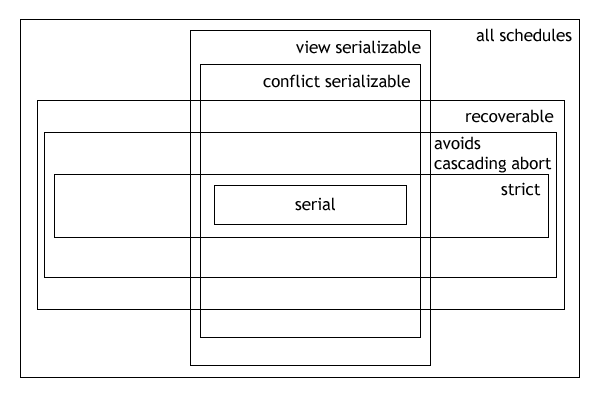
\includegraphics[scale=2]{rozvrhy.png}

Všeobecne zamerané DBMS využívajú najmä konflikt-sériovateľné striktné rozvrhy.
\end{frame}

\begin{frame}[fragile]{Rozvrhy}
Metódy na generovanie vyhovujúcich rozvrhov:
\begin{itemize}
\item multi-version concurrency control (MVCC)
\item dvojfázové zamykanie
\item časové pečiatky
\item validácia
\item \dots
\end{itemize}
\end{frame}

\begin{frame}[fragile]{Zámky}
Základnou technikou na generovanie konflikt-sériovateľných rozvrhov je použitie zámkov.
\alert{Zámky} môžu mať rôznu granularitu (záznam, celá tabuľka apod.). Typy zámkov:
\begin{itemize}
\item exkluzívne, na čítanie aj písanie (write lock)
\item zdieľané, len na čítanie (read lock)
\item upgrade lock atď.
\end{itemize}
Pred vykonaním operácie musí transakcia dostať zámok, ktorý jej umožní túto operáciu vykonať.
V minimalistickej verzii sa využijú len exkluzívne zámky, čiže prvá tx dostane prístup k objektu
a ostatné musia čakať (alebo budú abortnuté). Využitie zdieľaných zámkov (na čítanie) výrazne urýchli prácu systému,
v ktorom sa veľa číta a menej zapisuje.
\end{frame}


\begin{frame}[fragile]{Dvojfázové zamykanie}
Princíp dvojfázového zamykania (2PL) --- v prvej fáze transakcia zámky získava,
v druhej už len uvoľňuje. Pre dvojicu konfliktných operácií dochádza aj ku konfliktu zámkov
(nemôžu byť pridelené súčasne pre obe operácie).\\[2mm]

\blue{2PL generuje len konflikt-sériovateľné rozvrhy.}\\[2mm]

(Predpokladajme opak. Potom musí v precedenčnom grafe existovať cyklus,
povedzme $T_1 \rightarrow T_2 \rightarrow \dots \rightarrow T_1$.
Ak $T_i$ predchádza $T_j$, tak v príslušnej dvojici konfliktných operácií $T_j$ dostane zámok až po tom,
čo ho $T_i$ uvoľnila.
Potom však $T_1$ musí získať zámok až potom, čo ho uvoľnila, a to je spor s definíciou 2PL.)
\end{frame}


\begin{frame}[fragile]{Striktné dvojfázové zamykanie}
Ak pridáme k 2PL požiadavku na uvoľňovanie zámkov len pri commite (Strict 2PL), zníži to mieru paralelizmu
(niektoré rozvrhy generované 2PL už nebudú vyhovovať), ale zabezpečí generovanie striktných rozvrhov.\\[2mm]

Po zápise hodnoty do zdieľaného objektu bude transakcia držať exkluzívny zámok na tento objekt až do svojho commitu
a medzitým žiadna tx nemôže na tento objekt získať zámok, čiže žiaden dirty read (ani write) nemôže nastať.\\[2mm]

\scriptsize{Poznámka: Zdieľané zámky by bolo možné uvoľňovať aj skôr ako pri commite,
ale v~praxi to nevedie k pozorovateľnému zrýchleniu a pridáva overhead.
Uvoľňovanie zámkov pri commite je veľmi ľahké implementovať v podobe online algoritmu:
nepotrebujeme vidieť \uv{budúce} operácie tx, aby sme vedeli, kedy uvoľňovať zámky.}
\end{frame}

\begin{frame}[fragile]{Uviaznutie (deadlock)}
Rozvrh vytvorený 2PL môže viesť k \alert{deadlocku}:
vzniku cyklu transakcií, z ktorých každá čaká, kým predošlá uvoľní nejaký zámok, ktorý ona potrebuje.

Deadlock možno riešiť v momente, keď nastane (udržiavame graf čakajúcich transakcií a detegujeme v ňom cykly),
alebo jeho vzniku predchádzať niektorou zo známych metód
(idea je zachovať staršie transakcie, ktoré už nejakú prácu vykonali):
\begin{itemize}
\item \blue{wait-die}\\ (ak novšia tx žiada zámok od staršej, abortneme novšiu);
\item \blue{wound-wait}\\ (ak staršia tx žiada zámok od novšej, spôsobí jej abort).
\end{itemize}
\end{frame}



\begin{frame}[fragile]{Izolácia transakcií podľa SQL štandardu}
Štandard SQL vychádza z neželaných javov pri paralelnom behu transakcií.
\begin{itemize}
\item \alert{dirty read}
\item \alert{nonrepeatable read} (tx prečíta 2x po sebe ten istý záznam, ale dostane rôzne výsledky)
\item \alert{phantom read} (tx si vyžiada 2x záznamy určené tou istou podmienkou, ale dostane rôzne výsledky)
\item \alert{serialization anomaly} (výsledok rozvrhu niekoľkých tx nezodpovedá žiadnemu ich sériovému rozvrhu)
\end{itemize}
\end{frame}

\begin{frame}[fragile]{Izolácia transakcií podľa SQL štandardu}
Štandardné úrovne izolácie a ich implementácia v PostgreSQL:
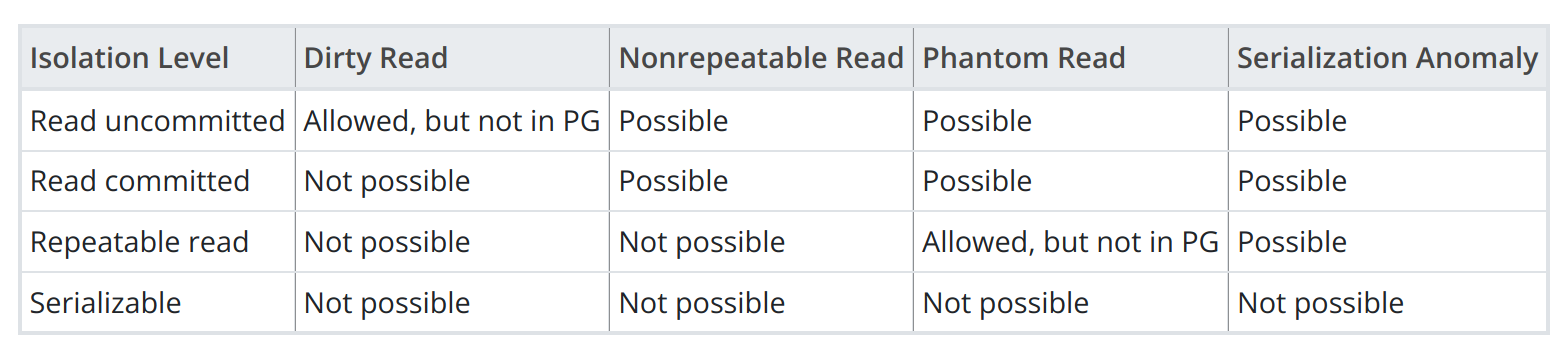
\includegraphics[scale=.2]{isolationLevels.png}\\[2mm]

Default by mal byť podľa štandardu \verb|SERIALIZABLE|, ale pre väčšinu DBMS to tak nie je.
Úroveň izolácie si vie transakcia zvoliť na začiatku, napr.
\begin{alltt}
  BEGIN TRANSACTION ISOLATION LEVEL REPEATABLE READ;
\end{alltt}

Existujú aj ďalšie nastavenia transakcií, napr. \verb|READ ONLY|.
\end{frame}

% General concepts: https://15721.courses.cs.cmu.edu/spring2018/notes/05-mvcc1.pdf
\begin{frame}{MVCC --- viac verzií toho istého riadka}
\begin{itemize}
\item DBMS uchováva viac verzií toho istého riadka; staršiu verziu môže ešte potrebovať súbežné čítanie.
\item \alert{Snapshot} určuje, ktoré verzie má čítanie vidieť.
Je to logický pohľad, nie fyzická kópia celej databázy.
\item Čítanie staršej verzie umožňuje pokračovať aj počas zmien vykonávaných inou transakciou.
\item Konflikty medzi zápismi stále treba riešiť.
Samotné MVCC neurčuje úroveň izolácie ani nezaručuje sériovateľnosť.
\end{itemize}
\end{frame}

% Multiversion serialization graphs: Ports and Grittner, Section 3.1.
% https://arxiv.org/abs/1208.4179
\begin{frame}{MVCC a sériovateľnosť}
\begin{itemize}
\item Hrana $T_1\to T_2$ v grafe závislostí znamená,
že $T_1$ musí v zodpovedajúcom sériovom poradí predchádzať $T_2$.
\item Zohľadňujeme čítania aj zápisy a to, ktorá verzia bola čítaná.
Ak konkrétne čítanie v $T_1$ použije verziu riadka staršiu než tú, ktorú zapíše $T_2$,
vzniká požiadavka $T_1\to T_2$.
\end{itemize}

\begin{center}
\begin{tikzpicture}
\node (t1) at (0,0) {$T_1$};
\node (t2) at (2.5,0) {$T_2$};
\node (t3) at (5,0) {$T_3$};
\draw[->] (t1) -- (t2);
\draw[->] (t2) -- (t3);
\draw[->] (t3) to[bend left=30] (t1);
\end{tikzpicture}
\end{center}

\begin{itemize}
\item Bez cyklu dá topologické usporiadanie grafu commitnutých transakcií
zodpovedajúce sériové poradie.
Sériovateľnosť môžeme zabezpečiť abortovaním transakcií,
ktoré by vytvorili cyklus.
\end{itemize}
\end{frame}

% https://www.postgresql.org/docs/15/transaction-iso.html
% https://www.postgresql.org/docs/15/routine-vacuuming.html
\begin{frame}[fragile]{MVCC v PostgreSQL}
\begin{itemize}
\item Predvolený \verb|READ COMMITTED|: bežný \verb|SELECT| nevidí necommitnuté zmeny iných transakcií.
Po commite inej transakcie môže náš ďalší \verb|SELECT| vidieť jej zmeny.
Už bežiaci \verb|SELECT| svoj snapshot nemení.
\item \verb|REPEATABLE READ|: snapshot zmien ostatných transakcií sa určí pri prvom dotaze
alebo zmene dát a počas transakcie sa už nemení.
\item V oboch režimoch transakcia navyše vidí svoje zmeny z predchádzajúcich príkazov,
aj keď ich ešte necommitla.
\item Súbežné zápisy do rovnakého riadka môžu viesť k čakaniu alebo abortu, aj pred commitom.
\item Nepotrebné staré verzie odstraňuje \verb|VACUUM|;
\verb|autovacuum| túto údržbu automatizuje.
\end{itemize}
\end{frame}

% Naive repeated cycle checking; n and m bound the graph size over the interval.
% Full graph tracking versus SSI: Ports and Grittner, Sections 3.3 and 6.
% https://arxiv.org/abs/1208.4179
\begin{frame}{Cena naivnej kontroly grafu}
\begin{itemize}
\item Graf má najviac $n$ transakcií a $m$ hrán.
\item Po pridaní každej novej hrany môžeme znovu vyhľadať cyklus v celom grafe:
\end{itemize}
\[
\underbrace{O(n+m)}_{\text{jeden test}},\qquad
\underbrace{O\bigl(k(n+m)\bigr)}_{\text{$k$ nových hrán}}.
\]
\begin{itemize}
\item Úplná evidencia grafu a kontroly cyklov sa pre PostgreSQL ukázali ako príliš nákladné.
Používa preto lacnejšiu konzervatívnu kontrolu, ktorá môže abortovať aj transakciu,
ktorej abort by nebol nevyhnutný.
\end{itemize}
\end{frame}

\begin{frame}[fragile]{MVCC a sériovateľnosť v PostgreSQL}
Pri \verb|SERIALIZABLE| sleduje PostgreSQL dve nadväzujúce závislosti
\[
T_1\longrightarrow T_2\longrightarrow T_3.
\]
\begin{itemize}
\item Obe hrany: transakcia čítala staršiu verziu než tú, ktorú zapísala ďalšia transakcia.
Takýto vzor musí obsahovať každý problematický cyklus pri snapshot isolation.
\item Kontrola zohľadní aj poradie commitov. V nebezpečnom prípade spravidla abortuje $T_2$;
ak $T_2$ aj $T_3$ už commitli, zostáva abortovať $T_1$.
\item Nemusí evidovať všetky typy hrán ani prehľadávať celý graf.
Kontrola je konzervatívna: niektoré aborty by neboli nevyhnutné.
\end{itemize}
Tento postup bol publikovaný v roku 2008; PostgreSQL ho používa od verzie 9.1 (2011).
% Ports and Grittner, Sections 3.3, 5.4: https://arxiv.org/abs/1208.4179
% https://github.com/postgres/postgres/blob/REL_15_STABLE/src/backend/storage/lmgr/predicate.c
\end{frame}

\begin{frame}[fragile]{Upozornenie}
Paralelné spracovanie môže viesť k vzniku \alert{nečakaných chýb}, za ktoré samotná tx nemôže a nevie ich ovplyvniť, napr.
{\scriptsize
\begin{alltt}
    ERROR:  could not serialize access due to concurrent update
\end{alltt}
}
K takýmto chybám dochádza v bežnej prevádzke zriedkavo, ale robustný program s tým musí počítať.
\end{frame}


\begin{frame}{Literatúra}
\begin{itemize}
\item {\scriptsize\href{https://arxiv.org/abs/cs/0701157}{A Critique of ANSI SQL Isolation Levels}}
\item {\scriptsize\url{https://cs186berkeley.net/notes/note11/}}
\item {\scriptsize\url{https://cs186berkeley.net/notes/note12/}}
\item {\scriptsize\url{https://www.db-book.com/slides-dir/PDF-dir/ch17.pdf}}
\item {\scriptsize\url{https://www.db-book.com/slides-dir/PDF-dir/ch18.pdf}}
\item {\scriptsize\url{https://www.db-book.com/slides-dir/PDF-dir/ch19.pdf}}
\item {\scriptsize\url{https://en.wikipedia.org/wiki/Database_transaction_scheduling}}
\item {\scriptsize\href{https://www.postgresql.org/docs/current/mvcc.html}{Transaction isolation in PostgreSQL}}
\item {\scriptsize\href{https://www.sqlite.org/isolation.html}{Transaction isolation in SQLite}}
\item {\scriptsize\href{https://tinyurl.com/nhk9659m}{A beginner’s guide to Phantom Read anomaly}}
\end{itemize}
\end{frame}


\begin{frame}{Na zamyslenie}
\begin{itemize}
\item Prečo chceme, aby rozvrhy boli ekvivalentné sériovým rozvrhom? A v akom zmysle majú byť ekvivalentné?
\item Je možné získať izoláciu transakcií na úrovni SERIALIZABLE (podľa SQL štandardu), ak využívame 2PL iba so zámkami na jednotlivé riadky?
\item Nájdite rozvrh, ktorý je konflikt-sériovateľný, ale nie je obnoviteľný.
\item Nájdite rozvrh, ktorý je obnoviteľný, ale nie je konflikt-sériovateľný.
\item Nájdite rozvrh, ktorý nie je obnoviteľný, ale dá sa generovať 2PL. Ukážte, že sa nedá generovať striktným 2PL.
\item Prečo v DBMS nie je zmysluplné implementovať 2PL (ale strikné 2PL je OK)? (Súvisí s pojmom \emph{online algorithm}.)
\end{itemize}
\end{frame}

\end{document}
